\documentclass[]{aiaa-tc} % insert '[draft]' option to show overfull boxes

 \title{Gradient-Based Optimization on Large Design Spaces with Graph-Based Problem Formulation In OpenMDAO}
        
\author{
  Tristan A. Hearn,%
     \thanks{Aerospace Engineer, MDAO Branch, Mail Stop 5-10, AIAA Member}
  \ Kenneth T. Moore,%
     \thanks{Senior Systems Engineer, MDAO Branch, Mail Stop 500-105, AIAA Senior Member} 
  \ Justin Gray,%
     \thanks{Aerospace Engineer, MDAO Branch, Mail Stop 5-11, AIAA Member}
   \\
  {\normalsize\itshape
  NASA Glenn Research Center, Cleveland, OH}  \\
 }

\AIAAconference{Multidisciplinary Design Optimization Specialist Conference}
\AIAAcopyright{\AIAAcopyrightD{2012}}


% Define commands to assure consistent treatment throughout document
\newcommand{\eqnref}[1]{(\ref{#1})}
\newcommand{\class}[1]{\texttt{#1}}
\newcommand{\package}[1]{\texttt{#1}}
\newcommand{\file}[1]{\texttt{#1}}
\newcommand{\BibTeX}{\textsc{Bib}\TeX}

\setlength{\abovecaptionskip}{0pt}
\setlength{\belowcaptionskip}{0pt}

\usepackage{setspace}

\usepackage{graphicx}
\usepackage{wrapfig}
\usepackage{caption} 
\usepackage{amsmath}
\usepackage{lscape}
\usepackage{hyperref}
\usepackage{minted}
\usepackage{color}
\usepackage{appendix}
\usepackage[section]{placeins}


\captionsetup[figure]{margin=5pt,font=small,labelfont=bf,textfont=bf,justification=justified,}
%\captionsetup[wrapfigure]{margin=5pt,font=small,labelfont=bf,justification=justified,singlelinecheck=off}
\captionsetup[table]{margin=5pt,font=small,labelfont=bf,textfont=bf,justification=justified,position=top}

\bibliographystyle{aiaa}

\usepackage{lettrine}
\usepackage{verbatim}

\begin{document}

  \maketitle
   
  \begin{abstract}

  \end{abstract}

  \section{Introduction}

    Many of today's the most interesting design problems involve very large design spaces with 100's or 1000's of 
    design variables. Large design spaces are often approached through the use of gradient based optimization 
    analytic derivatives to achieve highly scalable solution strategies. For instance, adjoint based gradient 
    methods have allowed CFD based shape optimization to tackle problems with 100's of design variables. [Cite Juan's Groups
    work here]. Coupled Aero-structural optimization is another area where gradient based optimization methods have 
    been employed. [Cite Martins groups work here]. Although these problems have large design spaces, 
    they include only a few disciplines (i.e. Geometry, Aerodynamics, Structures). The relative simplicity of 
    the problem formulation make it feasible to use custom implementations tailored to a specific problem. Naturally however, 
    this approach also limits the problem complexity that can be addressed with current MDAO methods. 

    On the other end of the spectrum, traditional systems analysis models can be composed of 10's to 100's of disciplines, 
    but usually work with lower fidelity analyses. These problems commonly contain a very high degree of interdisciplinary 
    coupling, while working with lower fidelity analyses. These more complex problem formulations are much more difficult to compute 
    analytic derivatives for at the system level, even if each discipline could provide its own partial derivatives. So many 
    problems are solved using a finite difference approach, which restricts the size of the design space. 

    If you placed complexity on the Y-axis and Fidelity on the X-axis, then the problem spectrum resemble the notional 
    cartoon in Figure \ref{fig:complexity_cartoon}. In this diagram, there is a gap between the lower and higher fidelity 
    type problems is indicative of the bifurcation in methods used to solve each type of problem currently. This gap begs the 
    question, ``How should you appraoch a problem of medium complexity and medium fidelity?'' We propose that the answer to this
    dilemma is to develop a more general manner of implementing MDAO problems that can be applied to any problem across the entire 
    space of complexity and fidelity.  

    \begin{figure}[!htb]
      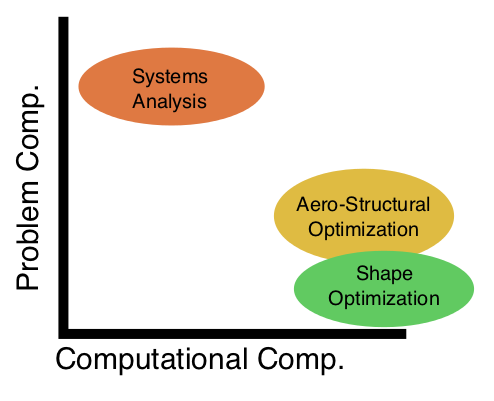
\includegraphics[width=.5\textwidth]{images/complexity_cartoon}
      \caption{ Notional spectrum of design problems currently being addressed. \label{fig:complexity_cartoon}}
    \end{figure}

    In this work we demonstrate how OpenMDAO, an open-source framework, such a general 
    solution to constructing and solving complex problems with large design spaces using the 
    same MDAO methods commonly applied to the the shape optimization and aero-structural optimization 
    problems. OpenMDAO achieves this by providing three key features: 

    \begin{enumerate}
      \item Automatic handling of arbitrary interdisciplinary coupling 
      \item Automatic formulation of gradients, including coupled derivatives, given arbitrary coupling
      \item Efficient operation in a high performance computing environment with distributed data
    \end{enumerate}

    \begin{comment}
      \begin{enumerate}
        \item Combining analytic derivatives with finite difference in a mixed derivatives environment
        \item Efficient solving for the coupled derivatives at the system level 
        \item Assembly of the full gradient from the partial derivatives of each discipline
        \item Flexbility via separation of problem formulation from solution strategy 
        \item Simple implementation for multi-point design problems
      \end{enumerate}
    \end{comment}

    To demonstrate these capabilities, we present two different problems representing different levels of 
    complexity and fidelity, solved within the OpenMDAO framework. The fist problem is the design of a small 
    satellite platform for taking weather measurements in the thermosphere, called CADRE. The CADRE problem has a 
    complex problem formulation with XX disciplines and over 25000 design variables, but is lower fidelity and can 
    be run on a single processor. This problem demonstrates that OpenMDAO successfully bridges the gap between shown 
    in Figure \ref{fig:complexity_cartoon}. The second problem is an aero-structural design of the Common Research 
    Model wing, using CFD and FEA. This problem shows that OpenMDAO can work with problems that demand higher fidelity 
    simulations with distributed data. 

  \section{Problem Formulation Graph}


    OpenMDAO maintains a central, monolithic, data connectivity graph between all 
    variables and components in the model, called the dependency graph. The graph utilizes the structure proposed by 
    Pate et. al \cite{graph_problem2013} and represents the complete problem formulation as 
    defined by the user. In a dependency graph each component and all variables of that component are 
    represented by nodes with directed edges between them describing their dependencies on each other. 

    In OpenMDAO when an input needed by one discipline is provided by the output of another. This is a dependency, and is represented 
    in a dependency graph containing nodes for the output and input, and an directional edge
    between them. It is clear that the upstream discipline must provide the output before the 
    downstream one can receive it, and this directional information is contained in the dependency
    graph.

    The main advantage of tight integration with a dependency graph is the availability of efficient
    algorithms for performing a number of functions that are useful for solving an MDAO problem.

      1. Determination of component execution order.
      2. Identification of cycles.
      3. Identification of parallel structures.
      4. Determination of driver subgraphs.
      
    The OpenMDAO framework uses a dependency graph to determine component execution order and to
    drive the process of invalidation, which finds the minimum set of components that needs to
    be re-executed when a set of inputs change. (ref: last OpenMDAO paper.) A dependency graph
    can also identify cycles in the graph, and hence a cycle in the dataflow that must be resolved
    by a solver. Similarly, the graph can also be used to examine the potential for parallelism at
    a component level.

    The determination of driver subgraphs is a capability that will be investigated in this paper.
    Consider an optimizer with n parameters, 1 objective, and m constraints. The relevant 
    subgraph of this problem is the set of component disciplines and their variable connection that
    lie within the subgraph between the parameters and the constraints and objective. This subgraph
    contains the components that execute when the optimizer requests a function evaluation. It is
    also useful for setting up and solving the coupled derivative system when the optimizer requests
    a gradient evaluation. For calculation of the coupled derivative in adjoint mode, further
    efficiency can be gained by using the subgraph that includes just the portion of the graph 
    between a single constraint and the parameters. Similarly for forward mode, the subgraph would
    include just the portion of the graph between a single parameter and the constraints/objective.

    [Intro to OpenMDAO paragraph]

    [Derivatives in OpenMDAO paragraph]


    \subsection{Fake Finite Difference}
    \subsection{Relevant Variable Identification}

  \section{CADRE Problem Formulation}

  \section{CADRE Results}

  \section{Aero-Structural Problem Formulation}

  \section{Aero-Structural Results}

  \section{Conclusion}
 
  \bibliography{references}

\end{document}
